% Seção 2: Tecnologias Habilitadoras do 5G

\section{Tecnologias Habilitadoras do 5G}
\subsection{Redes Definidas por Software (SDN)}

\begin{frame}
    \frametitle{Introdução ao SDN}

    \begin{itemize}
        \item \textbf{Definição}: Arquitetura de rede que separa o plano de controle do plano de dados.
        \item \textbf{Componentes Principais}: Aplicações de rede, controlador SDN, switches programáveis, interfaces.
        \item \textbf{Vantagens}: Flexibilidade, centralização do controle, automação.
    \end{itemize}
    \begin{figure}
        \centering
        \subfloat[Tradicional]{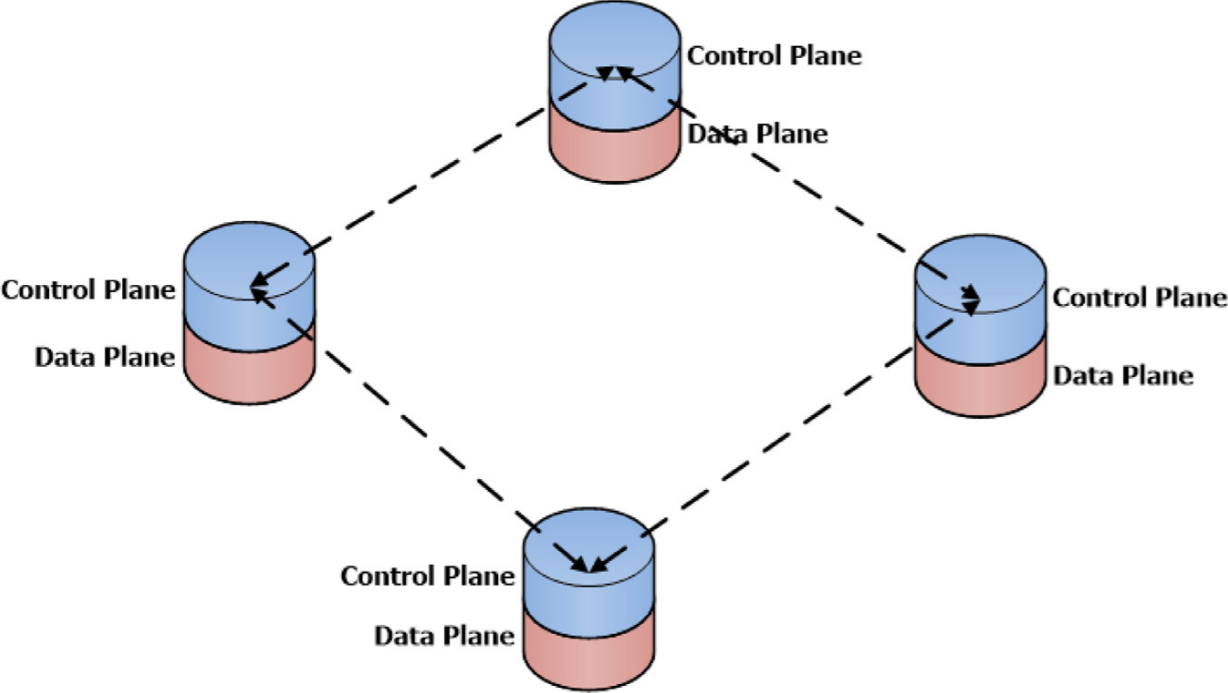
\includegraphics[width=0.45\linewidth]{figs/rede_tradicional.png}}\qquad
        \subfloat[SDN]{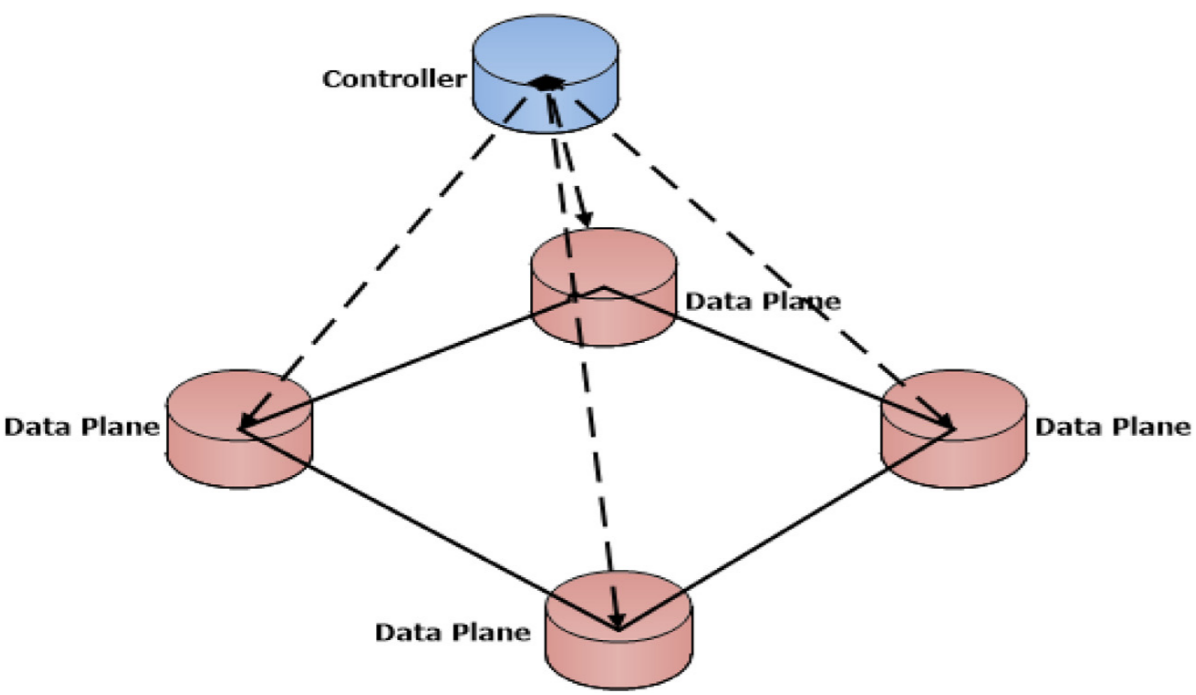
\includegraphics[width=0.45\linewidth]{figs/rede_sdn.png}}
        \caption{Redes tradicionais vs SDN\footcite{Plane_Separation}}
        \end{figure}
\end{frame}

\begin{frame}
    \frametitle{Componentes SDN}
    \begin{columns}
        \begin{column}{0.55\textwidth}
            \begin{itemize}
                \item \textbf{Plano de Aplicação}: Controle dos recursos via programação.
                \item \textbf{Plano de Controle}: Gerência centralizada dos recursos de rede.
                \item \textbf{Plano de Dados}: Dispositivos de comutação físicos ou virtuais.
                \item \textbf{Interfaces}: Comunicação entre os planos, ao norte (REST), sul (OpenFlow, P4), leste, oeste (API dos controladores).
        \end{itemize}            
        \end{column}
        \begin{column}{0.45\textwidth}
            \vspace{1cm}
            \begin{figure}[h]
                \centering
                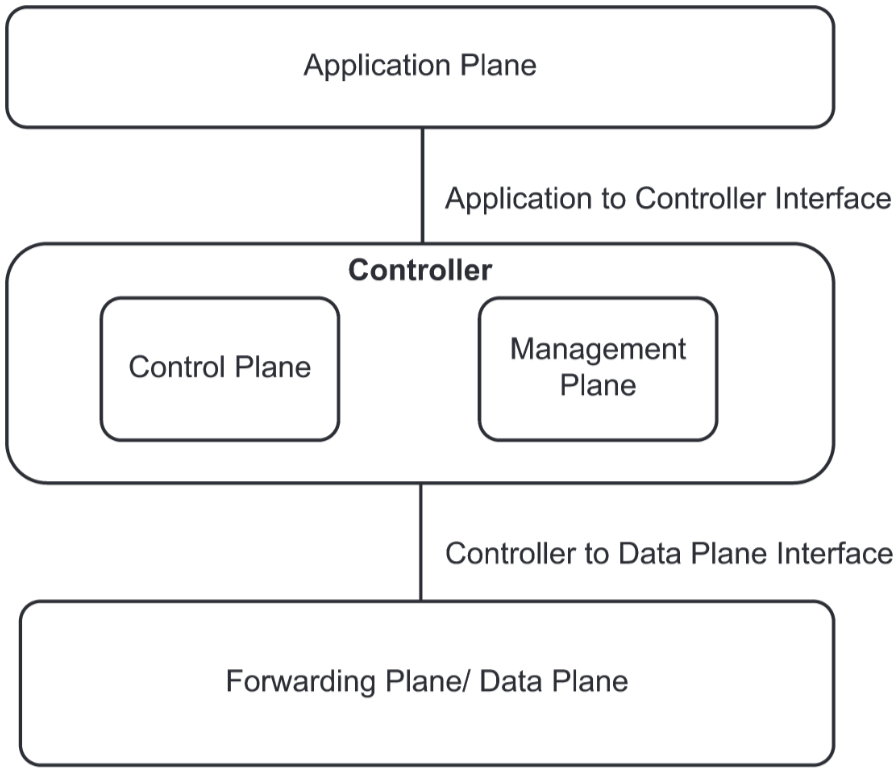
\includegraphics[width=\textwidth]{figs/SDN_arquitetura.png}
                \caption{Arquitetura SDN\footcite{Recommended_SDN_Wireless}}
            \end{figure}
        \end{column}
    \end{columns}
\end{frame}

\begin{frame}
    \frametitle{Integração SDN com 5G}
    \begin{itemize}
        \item \textbf{Automação de Redes}: Gerência dinâmica do tráfego e recursos.
        \item \textbf{Casos de Uso}: Redes IoT, redes industriais, redes de campus.
        \item \textbf{\textit{Network Slicing}}: Criação de fatias para diferentes serviços.
    \end{itemize}
\end{frame}

\subsection{Virtualização das Funções de Rede (NFV)}
\begin{frame}
    \frametitle{Introdução ao NFV}
    \begin{itemize}
        \item \textbf{Definição}: Abstração das funções de rede do hardware proprietário, executando-as em servidores padrão.
        \item \textbf{Componentes Principais}: VNF (Funções de Rede Virtualizadas), NFVI (Infraestrutura de Virtualização).
        \item \textbf{Vantagens}: Redução de custos, flexibilidade, rapidez na introdução de serviços.
    \end{itemize}
\end{frame}

\begin{frame}
    \frametitle{Integração NFV com 5G}
    \begin{itemize}
        \item \textbf{Virtualização do EPC (\textit{Evolved Packet Core})}: Gestão centralizada e flexível do core da rede.
        \item \textbf{vRAN (\textit{Virtualized Radio Access Network})}: Otimização da rede de acesso rádio.
        \item \textbf{\textit{Edge Computing}}: Suporte a aplicações de baixa latência e alta demanda.
    \end{itemize}
    \begin{figure}
        \centering
        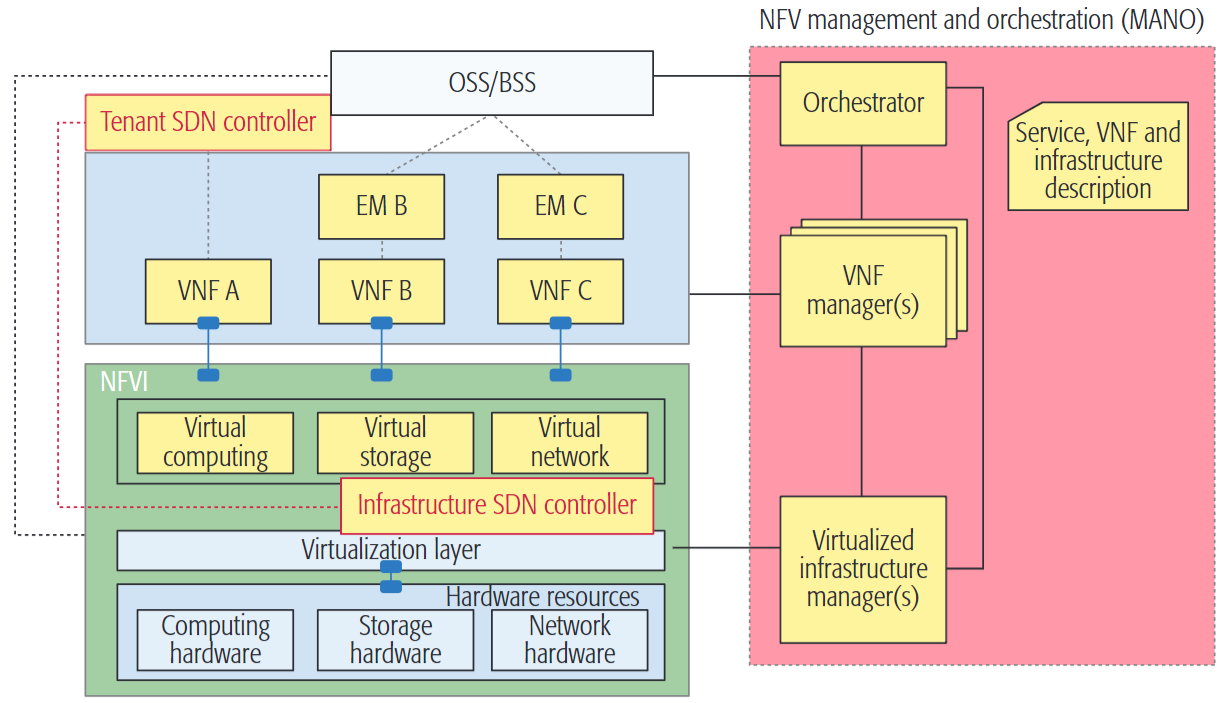
\includegraphics[width=0.6\linewidth]{figs/ArquiteturaNFV.png}
        \caption{Arquitetura geral NFV}
    \end{figure}
\end{frame}

\subsection{\textit{Network Slicing} (NS)}
\begin{frame}
    \frametitle{Introdução ao \textit{Network Slicing}}
    \begin{itemize}
        \item \textbf{Definição}: Técnica que permite a criação de múltiplas redes virtuais independentes sobre uma única infraestrutura física, otimizadas para atender diferentes requisitos de serviços e aplicações dentro de uma rede 5G.
        \item \textbf{Componentes Principais}: NFV e SDN.
        \item \textbf{Vantagens}: Garantir QoS, agilidade de implantação, personalizar e otimizar recursos de rede para diferentes serviços.
    \end{itemize}
\end{frame}

\begin{frame}{Integração NS com 5G}
    \begin{figure}[h]
        \centering
        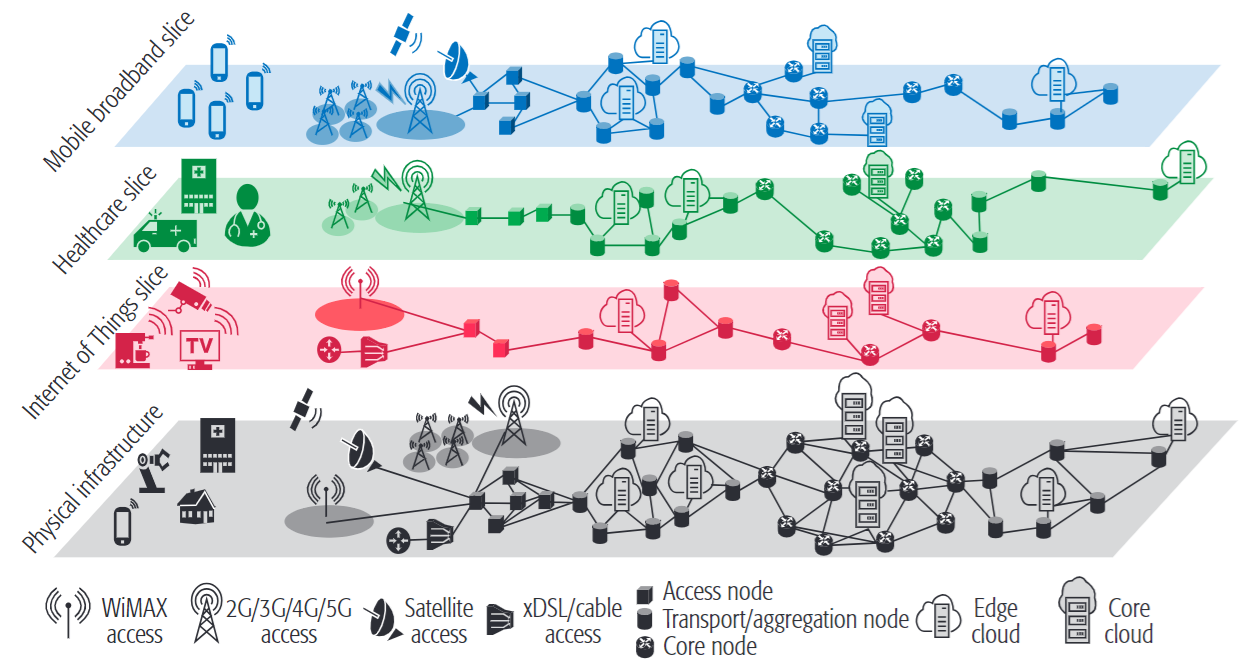
\includegraphics[width=\textwidth]{figs/Network_Slicing.png}
        \caption{Fatiamento de redes\footcite{Network_Slicing}}
    \end{figure}
\end{frame}